\section{Improvements in the high-level trigger system}

\graphicspath{{5_Outlook/Figures}}

As described in Sec.~\ref{subsec:trigger_system}, high-level trigger (HLT) in CMS is the last step of event selection before accepted events are saved for storage
and offline analysis.
The event selection at this step is done by reconstructing physics objects within the event, such as electrons, muons, jets, 
and missing transverse momentum (each defined in Sec.~\ref{sec:objects}).
Several identification criteria are applied on these reconstructed physics objects to select events of potential interest. The reconstruction of each
type of particle is described in~\cite{cms:hlt_paper}.

The event selection logic at HLT is structured around the concept of a \textit{HLT path}. Each HLT path is a sequence of processes running in a pre-defined order, which
reconstructs physics objects and applies selections on them. Typically every HLT path is defined to reconstruct a certain type of physics object (e.g. jets), and apply
selections on that object to decide whether the event should be kept or not. For the purposes of the VBF $\hinv$ analysis described in earlier sections of this thesis,
HLT paths that select events based on $\ptmiss$ are very important, since the $\hinv$ decays are expected to produce $\ptmiss$ in the final state. A discussion of how
$\ptmiss$ based triggers are used to collect data for the analysis is already given in Sec.~\ref{subsubsec:met_trigger_eff}. It should be noted that such $\ptmiss$-based triggers
are not only important for analyses targeting $\hinv$ signal, but they are commonly used for many analyses that search for Beyond the Standard Model (BSM) physics. Therefore,
improvements in the event selection of such HLT paths can play a crucial role for many analyses within the CMS experiment.

\subsection{Revisiting HF noise mitigation}
\label{subsec:hf_noise_hlt}

Extending the discussion in Sec.~\ref{subsec:hfnoise} to HLT paths which select events based on $\ptmiss$, 
it was observed that a large number of events with mismeasured HF jets are getting accepted by such HLT paths. 
As described in Sec.~\ref{subsec:hfnoise}, this is due to the creation of large $\ptmiss$ when the energy of one final state jet in QCD multijet
production events is mismeasured. This impacts a number of things:

\begin{itemize}
    \item Events with fake $\ptmiss$ are accepted and saved to offline storage. Such events would then require offline noise-cleaning treatment to be used in an analysis.
    \item The output event rate of $\ptmiss$ triggers are increased, due to events with mismeasured HF jets being accepted together with events with true $\ptmiss$.
\end{itemize}

Therefore, discrimination between a mismeasured HF jet and a well-identified jet at these HLT paths can play a crucial role to reject events that are not of interest.
This will also help decreasing the output rate coming from these paths, freeing up rates that could be used by other HLT paths in CMS. Expanding on the ideas introduced
in Sec.~\ref{subsec:hfnoise}, the jet shower shape variables are studied again at HLT reconstruction, and a jet-based filter is developed to increase the 
rate of rejection of events with mismeasured HF jets. The studies for the filter are outlined below, and the performance checks with these new $\ptmiss$ based paths
using Run3 data are shown in Sec.~\ref{subsec:trig_perf_check_run3}.

The studies conducted to develop the filter are identical to the studies described in Sec.~\ref{subsec:hfnoise}. 
The same jet shower shape variables are used to distinguish mismeasured jets from well-identified jets: $\sieie$, $\sipip$ and $\hfcss$. 
Jets are measured in ``physics-enriched'' and ``noise-enriched'' regions, where ``noise-enriched'' region refers to the events with a high-$\pt$ jet
recoiling against high $\ptmiss$, and ``physics-enriched'' region refers to the events with a high-$\pt$ jet recoiling against a well-identified photon.
One difference compared to the study described in Sec.~\ref{subsec:hfnoise} is that this study is restricted to jets which are reconstructed where the
noise is observed to be peaking, $2.99 < |\eta| < 3.25$. Since the studies were done before the start of Run3 data taking (2022), data taken in 2018 is used.
The jet shower shape variables in these two regions are shown in Fig.~\ref{fig:hf_variables_hlt}.

\begin{figure}[htbp]
    \centering
    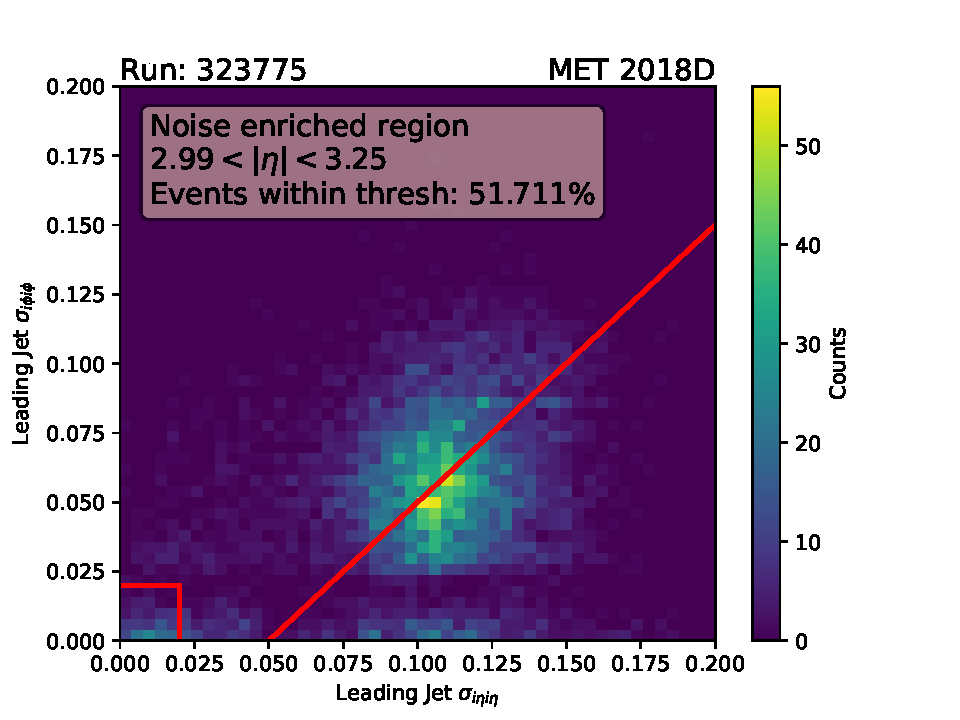
\includegraphics[width=0.45\textwidth]{HFFilter/merged_2022-04-11_hlt_11Apr22_MET_2018D/MET_2018D_sieie_sipip_ak4_abseta0_2_99_3_25_noise_enriched_mht_110.pdf}
    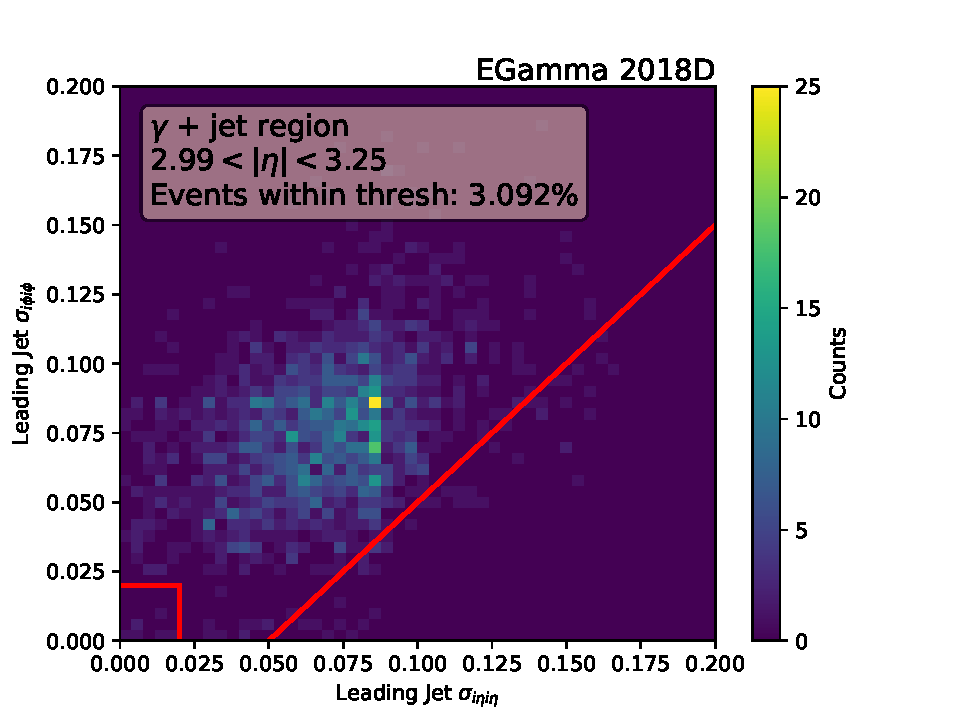
\includegraphics[width=0.45\textwidth]{HFFilter/merged_2022-04-12_hlt_11Apr22_EGamma_2018D/EGamma_2018D_sieie_sipip_ak4_abseta0_2_99_3_25_gammajet.pdf} \\
    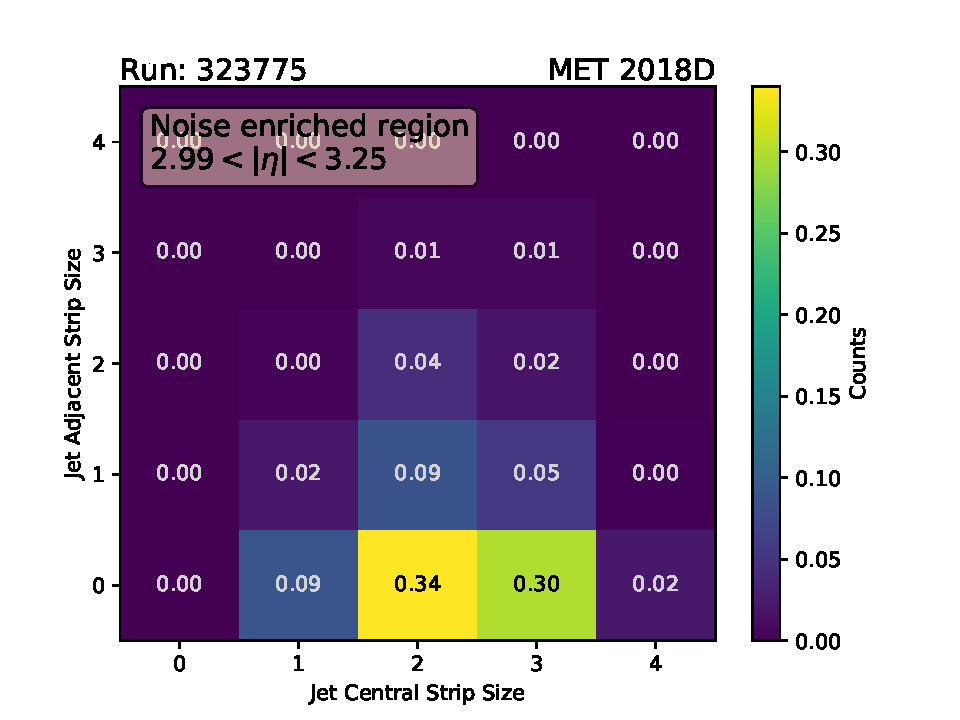
\includegraphics[width=0.45\textwidth]{HFFilter/merged_2022-04-11_hlt_11Apr22_MET_2018D/MET_2018D_cssize_adssize_ak4_abseta0_2_99_3_25_noise_enriched_mht_110.pdf}
    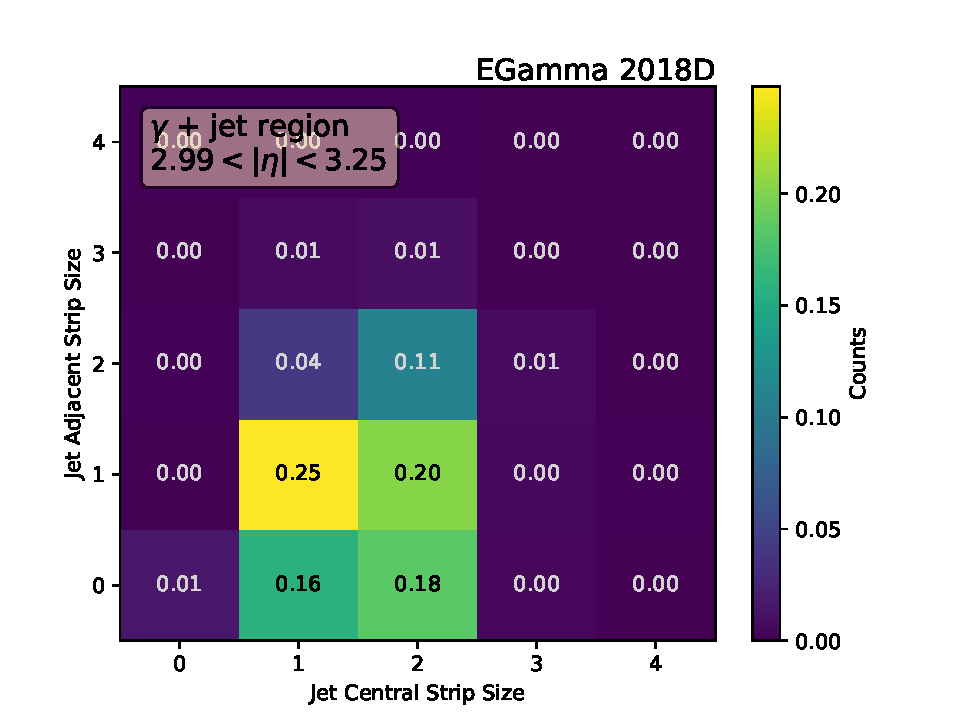
\includegraphics[width=0.45\textwidth]{HFFilter/merged_2022-04-12_hlt_11Apr22_EGamma_2018D/EGamma_2018D_cssize_adssize_ak4_abseta0_2_99_3_25_gammajet.pdf}
    \caption{The HF jet shower shape variables for noise-enriched (left) and physics-enriched regions (right).
    The top row shows the two-dimensional distributions of $\eta$ and $\phi$ width, $\sieie$ and $\sipip$. The red lines on these
    figures correspond to the filter applied to reject the jets, and the legend on top left quotes the percentage of jets that fail the requirements.
    The bottom row shows the distributions of central and adjacent strip sizes. Values of central strip size $\geq3$ are observed for mismeasured
    jets, and this variable is required to be $< 3$ as a part of the filter.}
    \label{fig:hf_variables_hlt}
\end{figure}

From Fig.~\ref{fig:hf_variables_hlt}, similar trends are observed compared to Figs.~\ref{fig:sieie_sipip_noise_enriched}, \ref{fig:sieie_sipip_physics_enriched}, 
\ref{fig:stripsize_noise_enriched} and \ref{fig:stripsize_phys_enriched}. Therefore, the following cuts were introduced to the HLT paths to identify a jet:

\begin{itemize}
    \item Jet should have $\sieie - \sipip < 0.05$
    \item Jet should not lie in the region where $\sieie < 0.02$ \& $\sipip < 0.02$
    \item Central strip size of the jet, $\hfcss < 3$
\end{itemize}

From Fig.~\ref{fig:hf_variables_hlt}, it can be observed that applying these cuts to the jets within $2.99 < |\eta| < 3.25$ can reject $\sim 50\%$ of mismeasured
jets, and the impact on well-reconstructed events (here, $\gamma$ + jet) is on the order of $1\%$. 

For the Run3 data taking at CMS experiment, a new set of HLT paths were included that utilize this jet filtering technique. The implementation is
done on HLT paths which cut on $\ptmiss$ and $\htmiss$, where $\htmiss$ is defined as the imbalance in total jet momenta,

\begin{equation}
    \htmiss = \left| \sum_{\mathrm{jet}} \ptvecjet \right| \quad ,
    \label{eq:htmiss_def}
\end{equation}
where the sum goes over jets with $\pt > 20$ GeV. The HF cuts are included in the HLT path such that if a jet fails the requirements, it will not be considered
in the $\htmiss$ calculation. This way, $\htmiss$ will be corrected from the impact of jets with mismeasured $\pt$ values, and the probability of such events
making it through the $\htmiss$ filter is lower.

\subsection{Performance checking with Run3 data}
\label{subsec:trig_perf_check_run3}

Using the most recent proton-proton collision data taken during Run3, the performance of the $\ptmiss$ and $\htmiss$ based paths with and without this filter is
monitored. Ideally, one would like to have the following performance constraints:

\begin{enumerate}
    \item For events with well identified physics objects, the loss of events caused by adding the filter should be minimal.
    \item For events with mismeasured jets, the rejection rate should be much larger, which would then translate to a reduction in rate.
\end{enumerate}

These performance considerations are explicitly checked using Run3 data. 
Two HLT paths are considered for this study, both paths require $\ptmissnomu > 120$ GeV and $\htmissnomu > 120$ GeV
to decide whether an event should be kept or not. The only difference between those two paths is the presence of the HF-filter derived in Sec.~\ref{subsec:hf_noise_hlt}.
These HLT paths are summarized in Tab.~\ref{tab:hlt_met_paths}.

\begin{table}[h!]
    \centering
    \caption{HLT paths used in this study. The left column shows the full name of the path and the right column shows whether the path has
    the HF-jet filter included as described in Sec.~\ref{subsec:hf_noise_hlt}. Both paths require $\ptmissnomu > 120$ GeV and $\htmissnomu > 120$ GeV
    to make a decision on whether to keep an event.}
    \label{tab:hlt_met_paths}
    \def\arraystretch{1.05}
    \begin{tabular}{l c}
        \hline
        HLT path name & Has HF jet-filter \\
        \hline
        HLT\_PFMETNoMu120\_PFMHTNoMu120\_IDTight           & No \\
        HLT\_PFMETNoMu120\_PFMHTNoMu120\_IDTight\_FilterHF & Yes \\
    \end{tabular}
\end{table}

\subsubsection{Impact on well-reconstructed events}

To check the loss of events due to the newly added HF-jet filter, efficiencies of the two paths in Tab.~\ref{tab:hlt_met_paths} are compared
on $\Wmnjets$ events. The events to consider in the efficiency measurement are selected by the following criteria:

\begin{itemize}
    \item Leading jet $\pt > 30$ GeV, leading jet must be tightly identified, according to the definition in Sec.~\ref{sec:objects_jets}.
    \item Events must pass a muon HLT path HLT\_IsoMu27, which requires a muon to be reconstructed with $\pt > 27$ GeV at HLT.
    \item Events must have a well-identified muon (reconstructed offline) with $\pt > 30$ GeV, which is tightly identified, as defined in Sec.~\ref{subsec:muons}.
\end{itemize}

The efficiency of the $\ptmissnomu$-based paths are measured as a function of recoil, which corresponds to $\pt$ of the W boson (see Sec.~\ref{subsec:objects_met_recoil}). 
The efficiencies are shown in Fig.~\ref{fig:filterhf_efficiency}, where the left-hand side plot shows the efficiency of the HLT path without the HF-jet filter, and the right-hand side plot
shows the efficiency of the other path with the filter. To model the turn-on behavior of the efficiencies, a sigmoid function is fit to both curves, which is defined as follows:

\begin{equation}
    f(x) = \frac{1}{1 + e^{-(x - \mu)/\sigma}} \quad ,
\end{equation}
where $\mu$ and $\sigma$ are determined from the best-fit to the data. The best-fit $\mu$ and $\sigma$ parameters are also shown in the legend for each plot.
It can be observed that for the two paths, the efficiencies are found to be almost identical, hence
supporting the fact that the loss of well-reconstructed events from the HF-filter is very minimal.  

\begin{figure}[htbp]
    \centering
    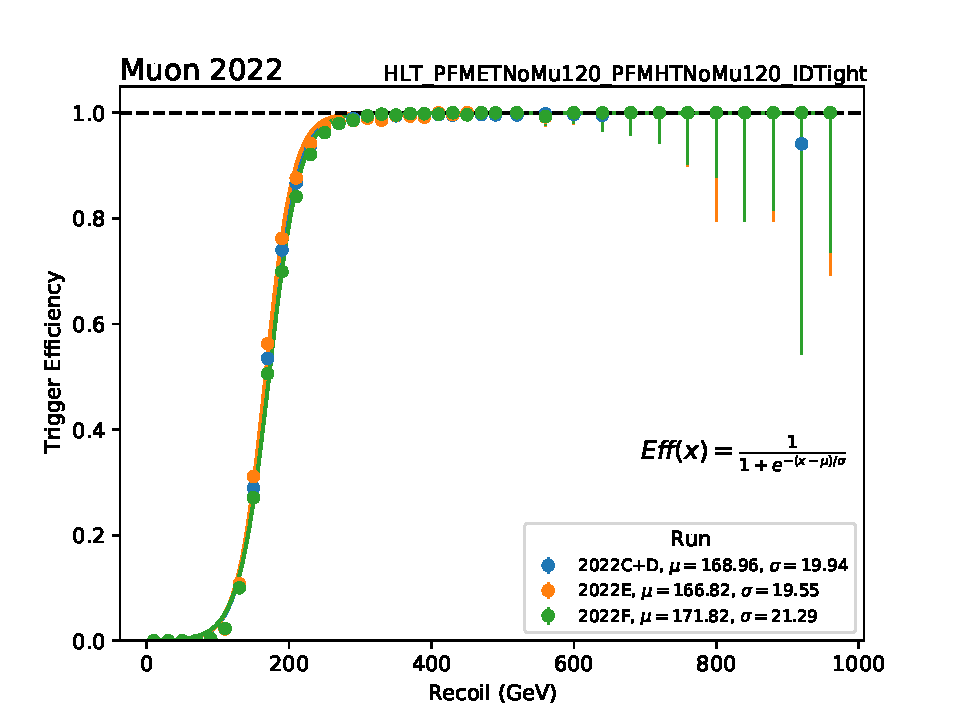
\includegraphics[width=0.45\textwidth]{HFFilter/merged_2022-10-27_hlt_Muon_2022_JMEtriggers/turnons_tr_metnomu.pdf}
    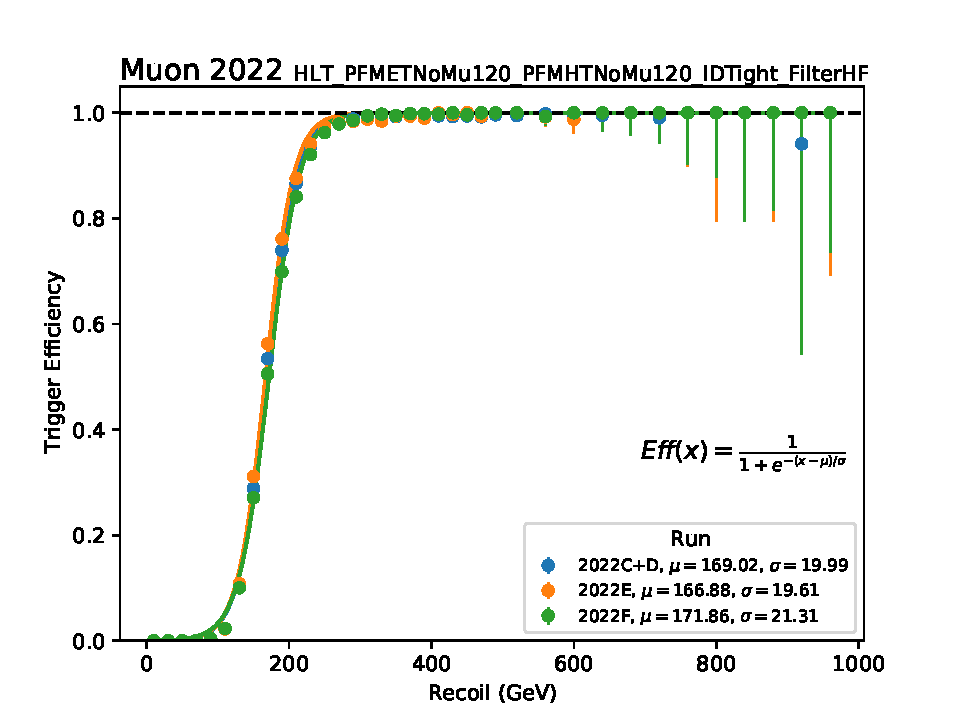
\includegraphics[width=0.45\textwidth]{HFFilter/merged_2022-10-27_hlt_Muon_2022_JMEtriggers/turnons_tr_metnomu_filterhf.pdf}
    \caption{Efficiency of the $\ptmissnomu$ based HLT paths without (left) and with (right) the HF-filter. To each efficiency curve, a sigmoid function is fit
    to describe the turn-on behavior. The best-fit parameters $\mu$ and $\sigma$ are shown in the legend, located on the bottom right of each plot. Different curves
    represent different data taking periods within 2022.
    It can be observed that the two efficiencies are almost identical, hence supporting the fact that the loss of well-reconstructed 
    events from the HF-filter is very minimal.}
    \label{fig:filterhf_efficiency}
\end{figure}

\subsubsection{Impact on output rate}

To check the impact of the HF-jet filter on the output rate, events that are accepted by the two paths in Tab.~\ref{tab:hlt_met_paths} are examined. Fig.~\ref{fig:filterhf_rate}
shows the number of events passing the two paths, as a function of $\eta$ of their leading jet. Note that events with leading jet $\pt > 30$ GeV are considered. 
The blue curve corresponds to events passing the HLT path without the filter, and the orange curve corresponds to the path with the filter. Finally, the ratio pad at the bottom
gives the ratio between the orange and blue curves. It can observed that, close to an additional $50\%$ of events near $3<|\eta|<3.25$ are rejected 
with the HF-filter\footnote{Looking at Fig.~\ref{fig:hf_variables_hlt}, the $\approx 50\%$ rejection quoted here should not come as a big surprise.
Based on studies with the data taken in 2018, an approximate $50\%$ reduction of events where the leading-$\pt$ jet lies within $3 < |\eta| < 3.25$
was already estimated.}. 
This reduction of events is found to be corresonding to about $10\%$ overall reduction in rate of the HLT paths where the filter is introduced. It should also be noted that
outside the region where the leading jet is within $3 < |\eta| < 3.25$, the impact due to the HF-jet filter is either $0$ or very small. The small impact in this case comes from
events where another jet with high $\pt$ exists in the forward region and fails the HF cuts, resulting in the event failing the trigger.

\begin{figure}[htbp]
    \centering
    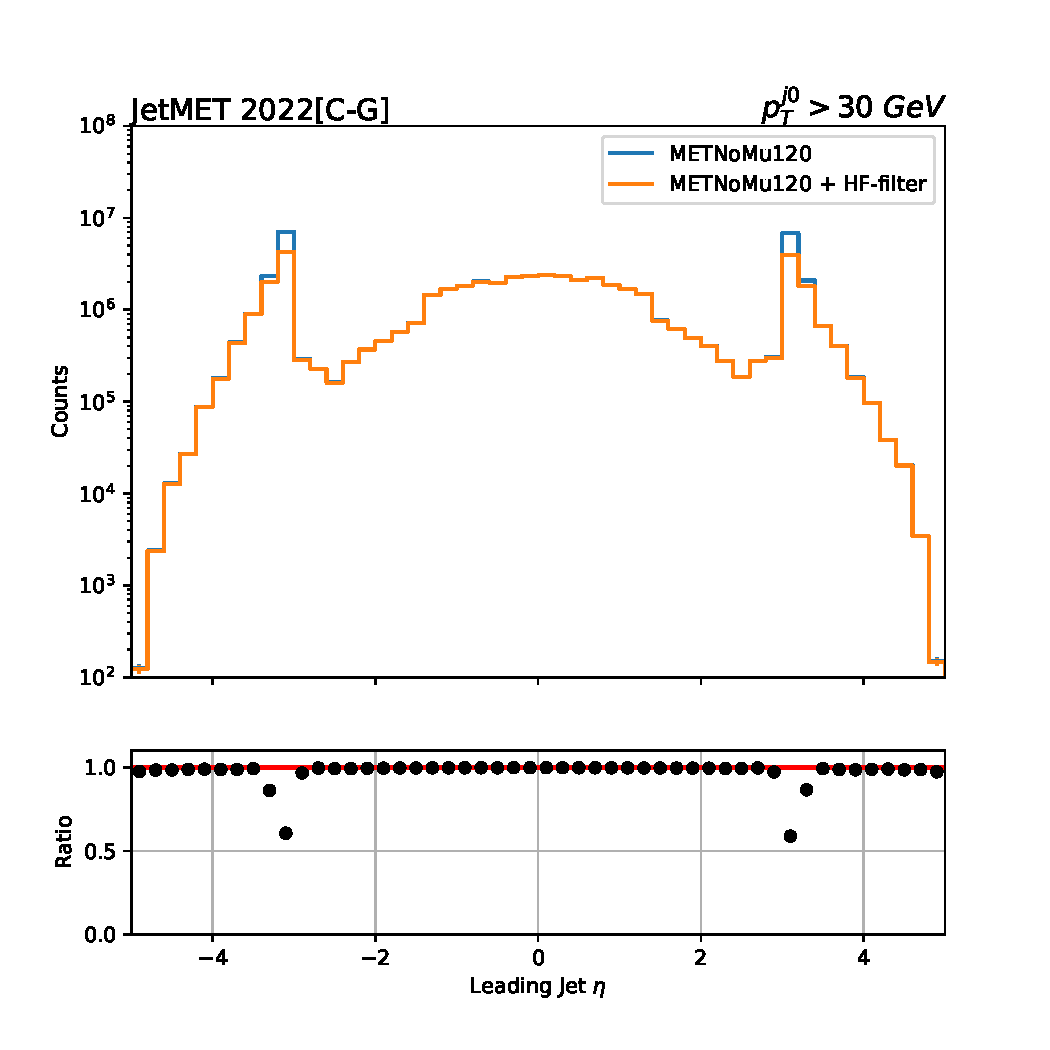
\includegraphics[width=0.7\textwidth]{HFFilter/merged_2023-02-10_hlt_full_JetMET_2022_run/ak4_eta0_filterhf.pdf}    
    \caption{Number of events passing the $\ptmissnomu$-based path with (orange) and without (blue) the HF-filter, as a function of $\eta$ of the highest-$\pt$ jet in the event.
    Note that events with leading jet $\pt > 30$ GeV are considered. The ratio pad at the bottom shows the ratio between orange and blue curves, hence effectively showing the additional
    rejection of events due to the new HF-jet filter.}
    \label{fig:filterhf_rate}
\end{figure}

\clearpage